\documentclass{standalone}


\begin{document}

\subsection[Pipeline]{DNetPRO in Snakemake}\label{implementation:snakemake}

The starting (silent) hypothesis done up to now is that we want to run the \textsf{DNetPRO} algorithm on a single dataset (or better on a single Hold-Out subdivision of data).
On this configuration it is legal to stress as much as possible the available computational resources and parallelize each step of the algorithm.

If we want to use our algorithm into a larger pipeline, in which we compare the results obtained over a Cross-Validation, we have to re-think about the parallelization done.
In this case, each fold of the cross validation can be interpreted as an independent task and, following the main programming rule \emph{\quotes{parallelize the outer, vectorize the inner}}, we should spawn a thread for each fold and perform the couple evaluation in sequential mode.
Certainly, the optimal solution would be to separate our jobs across a wide range of inter-connected computers, performing the same computation in parallel, but it would required to implement our hybrid (\textsf{C++} and \textsf{Python}) pipeline into a Message Passing Interface (MPI) environment.

The easier solution to overcome all these problems can be obtained using a set of \textsf{SnakeMake}~\cite{snakemake} rules.
\textsf{SnakeMake} is an intermediate language between \textsf{Python} and \textsf{Make}.
Its syntax is almost like the \textsf{Make} language, but with the help of the easier and powerful \textsf{Python} functions.
It is widely used in bioinformatics pipeline parallelization, since it can be easily applied over single or multi-cluster environments (master-slave scheme) with a simple change of command line.

\begin{center}
\begin{figure}[htbp]
\hspace{-2cm}
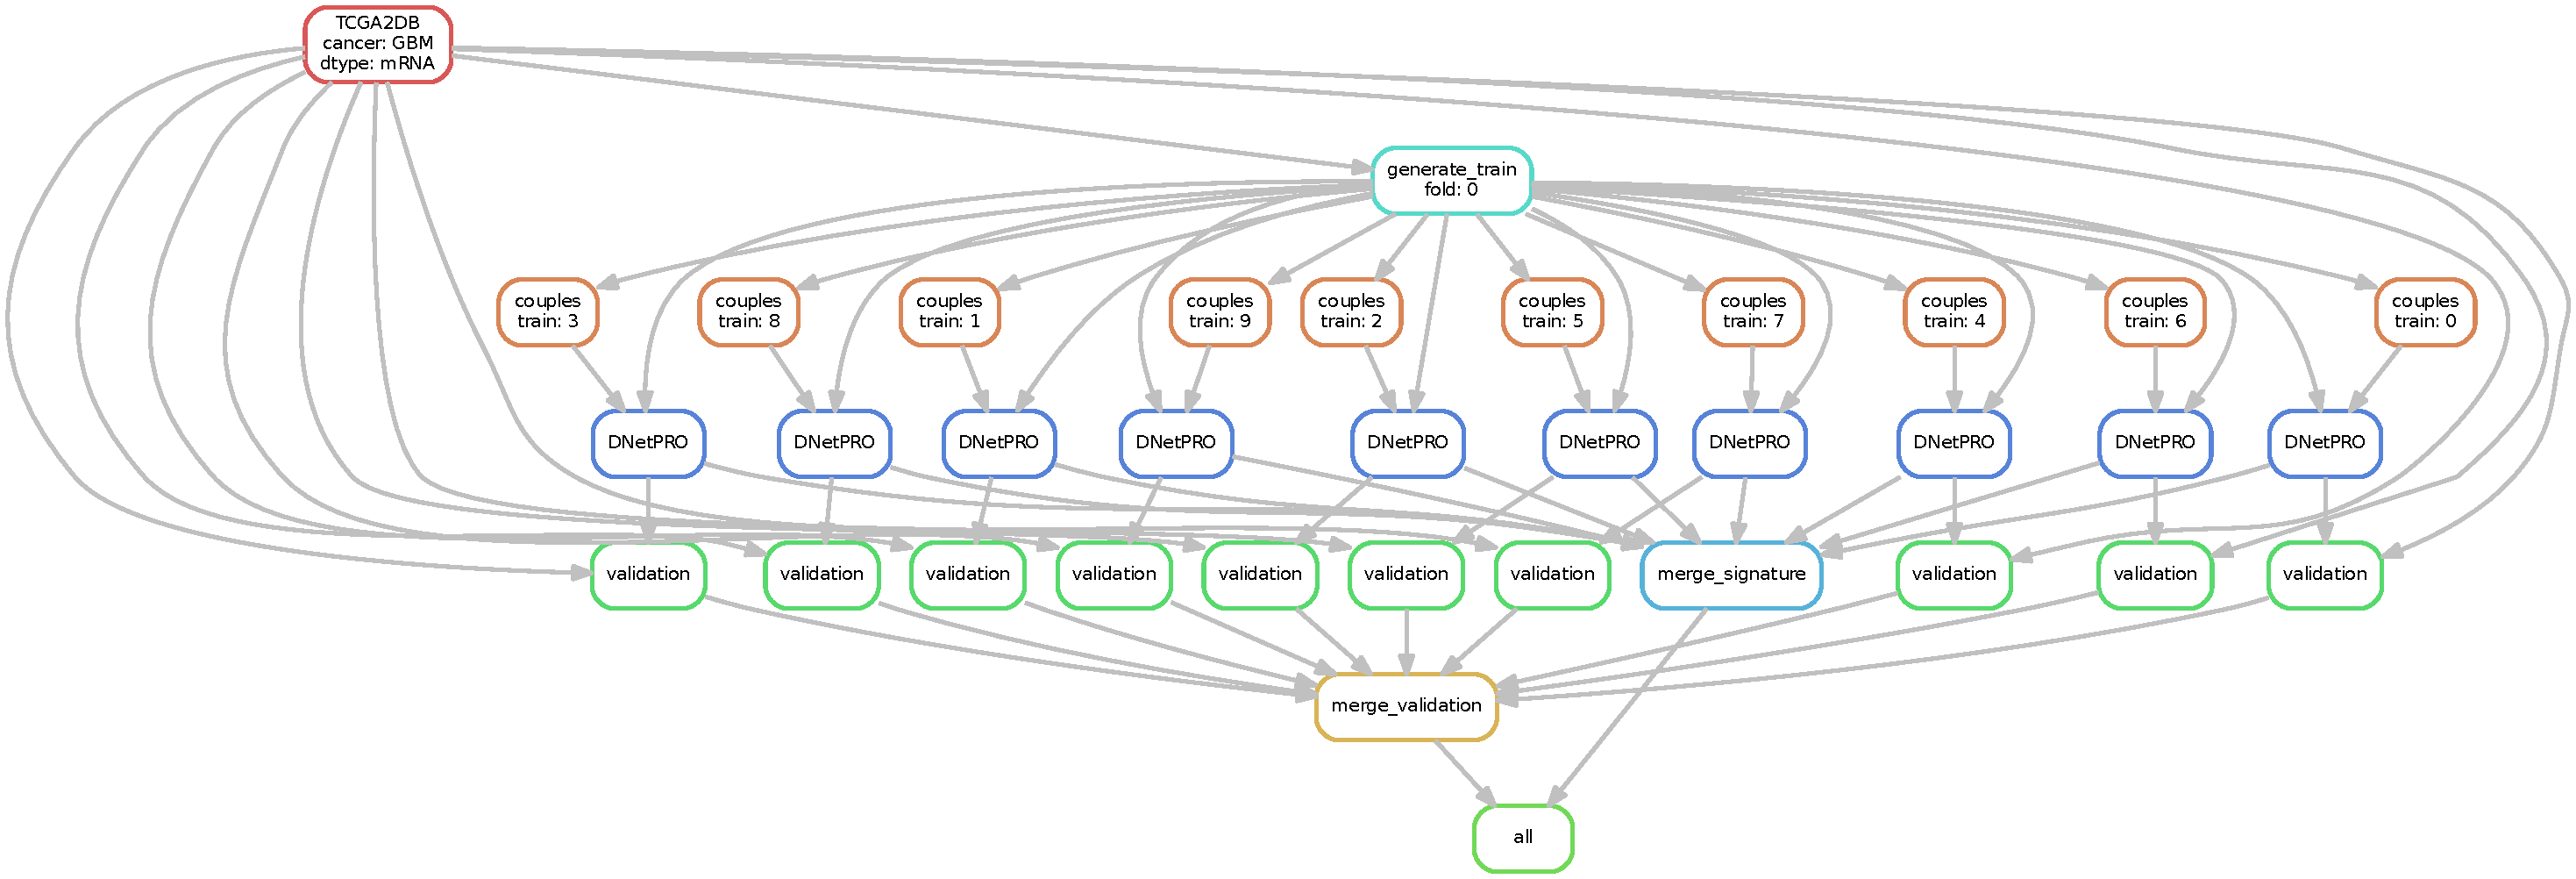
\includegraphics[width=1.3\textwidth]{qdanet_pipe_single.pdf}
\caption{Example of \textsf{DNetPRO} pipeline on a single cross validation.
It is highlighted the independence of each fold from each other.
This scheme shows a possible distribution of the jobs on a multi-threading architecture or for a distributed computing architecture.
The second case allows further parallelizations (hidden in the graph) applied to each internal step (e.g. the evaluation of each pair of genes).
}
\label{fig:dnet_workflow}
\end{figure}
\end{center}

So, to improve the scalability of our algorithm we implemented the benchmark pipeline scheme using \textsf{Snakemake} rules and a work-flow example for a single cross-validation is shown in Fig.~\ref{fig:dnet_workflow}.
In this case, each step of Fig.~\ref{fig:dnet_workflow} can be performed by a different computer-unit, preserving the multi-threading steps with a maximum scalability and possibility to enlarge the problem size (number of variables).


\end{document}
